\documentclass[%
 reprint,
 superscriptaddress,
 amsmath,
 amssymb,
 prl,
]{revtex4-1}

\usepackage{graphicx}% Include figure files
\usepackage{dcolumn}% Align table columns on decimal point
\usepackage{bm}% bold math
\usepackage{color}

\begin{document}

\title{Stabilisation of the Arrival Time of a Relativistic Electron Beam to 
the 50~fs Level}

\author{J.~Roberts}
\email{Corresponding author Jack.Roberts@cern.ch}
\affiliation{John Adams Institute (JAI), University of Oxford, Denys Wilkinson 
Building, Keble Road, Oxford, OX1 3RH, United Kingdom}
\affiliation{The European Organization for Nuclear Research (CERN), Geneva 23, 
CH-1211, Switzerland}

\author{P.~Skowronski}
\affiliation{The European Organization for Nuclear Research (CERN), Geneva 23, 
	CH-1211, Switzerland}

\author{P.N.~Burrows}
\affiliation{John Adams Institute (JAI), University of Oxford, Denys Wilkinson 
Building, Keble Road, Oxford, OX1 3RH, United Kingdom}

\author{G.B.~Christian}
\affiliation{John Adams Institute (JAI), University of Oxford, Denys Wilkinson 
Building, Keble Road, Oxford, OX1 3RH, United Kingdom}

\author{R.~Corsini}
\affiliation{The European Organization for Nuclear Research (CERN), Geneva 23, 
CH-1211, Switzerland}

\author{A.~Ghigo}
\affiliation{Laboratori Nazionali di Frascati (LNFN), Via Enrico Fermi, 40, 
00044 
Frascati RM, Italy}

\author{F.~Marcellini}
\affiliation{Laboratori Nazionali di Frascati (LNFN), Via Enrico Fermi, 40, 
00044 
Frascati RM, Italy}

\author{C.~Perry}
\affiliation{John Adams Institute (JAI), University of Oxford, Denys Wilkinson 
Building, Keble Road, Oxford, OX1 3RH, United Kingdom}


\date{\today}

\begin{abstract}
CLIC, a proposed future linear electron-positron collider, and other machines 
such as XFELs, place tight tolerances on the phase stabilities of their beams. 
CLIC proposes the use of a novel, high bandwidth and low latency, `phase 
feedforward' system required to achieve a phase stability of 
\(0.2^\circ\)~at~12~GHz, or about 50~fs. This work documents the results from 
operation of a prototype phase feedforward system at the CLIC test facility 
CTF3, with \(>23\)~MHz bandwidth and a total hardware latency of 100~ns. New 
phase monitors with 30~fs resolution, 20~kW amplifiers, 
and electromagnetic kickers have been designed and installed for the system. 
The system utilises a dog-leg chicane in the beamline, for which a dedicated 
optics have been created and commissioned. The prototype has demonstrated 
CLIC-level phase stability, reducing an initial rms phase variation of 
\(0.92\pm0.04^\circ\) to \(0.20\pm0.01^\circ\).
\end{abstract}

\maketitle

%%

High-energy linear electron-positron colliders have been proposed as 
next-generation particle accelerators for exploring the subatomic world with 
extreme precision. They will provide sensitivity to new physics processes, 
beyond those described by the Standard Model (SM) of elementary particle 
interactions, at mass scales that can exceed the eventual reach of the CERN 
Large Hadron Collider (LHC) by more than an order of magnitude. 

The Compact Linear Collider (CLIC) has been proposed ~\cite{CLICCDR} as a 
particle physics facility for the annihilation of electrons and positrons at 
centre-of-mass energies of up to 3 TeV. CLIC is the most technologically mature 
concept of a high-energy lepton collider for enabling direct searches for new 
physics processes in the multi-TeV energy regime. This energy reach, combined 
with high-luminosity of the electron-positron collisions, will also enable 
precise measurements of properties of the Higgs boson~\cite{CLIC-Higgs} and the 
top quark, and provide sensitivity to beyond-SM phenomena at mass scales of up 
to 10-100 TeV in some cases~\cite{CLIC-staging}.

The CLIC design employs the novel concept of high power generation at 
radio-frequency (RF) by decelerating an electron ‘drive beam’ and utilising 
that power to accelerate the main electron and positron beams to the desired 
high energies. The CLIC drive-beam concept is shown schematically in 
Fig.~\ref{fig:CLICLayout}; 50 deceleration sections are required for a 3 TeV 
electron-positron collider. At the decelerators the drive beam comprises a 
240~ns-long pulse of 2.4~GeV electrons bunched with a frequency of c. 12~GHz; 
the pulse repetition rate is 50~Hz.

A major challenge for this drive-beam acceleration concept is 
the synchronisation of the arrival of the drive and main beams at the 
power-extraction structures to an exceptional level of temporal accuracy. The 
arrival times need to be synchronised to better than 50~fs in order to limit 
the loss of luminosity, resulting from subsequent mis-acceleration of the main 
beams, to less than 1\% of the design value~\cite{Gerber2015}. Other types of 
novel particle accelerator, for example X-ray free-electron lasers, also 
demand a high degree of beam arrival-time stability w.r.t. an 
externally-applied laser beam for the purpose of ‘seeding’ of X-ray lasing from 
the electron beam. \textcolor{green}{An RF phase and amplitude stabilisation 
scheme using 
electro-optic beam arrival time monitors in this context was reported 
in~\cite{flashPRL}.}

\begin{figure}
	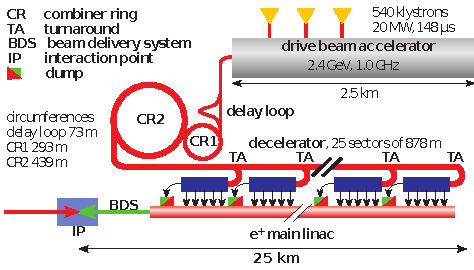
\includegraphics[width=\columnwidth]{figs/alt/clicLayout_cut_new}
	\caption{\label{fig:CLICLayout} Schematic of the CLIC two beam acceleration 
	concept.
	}
\end{figure}


Throughout this paper we use the equivalent 
term longitudinal ‘phase’ to refer to the beam time coordinate; 50~fs temporal 
stability is equivalent to \(0.2^\circ\) phase stability at 12~GHz RF. In the 
CLIC design the incoming drive-beam phase stability cannot be guaranteed to be 
better than \(2^\circ\)~\cite{CLICCDR}. A correction mechanism to improve the 
phase stability by an order of magnitude is 
therefore required and must be applied to the full drive beam pulse with a 
bandwidth exceeding 17.5~MHz~\cite{Gerber2015}. 
%Higher frequency errors are filtered as a consequence of the 
%drive beam recombination process, and by the accelerating structures 
%\cite{Gerber2015}.

The design calls for a `phase feed-forward' (PFF) system to measure the 
incoming beam phase and provide a derived correction to the same beam pulse 
after it has traversed the turnaround loop (TA in Fig.~\ref{fig:CLICLayout}). A 
PFF system will be installed in each deceleration section. The correction is 
provided by electromagnetic kickers in a 4-bend chicane: bunches arriving 
early (late) in time have their path through the chicane lengthened (shortened) 
respectively. A particular challenge is that the PFF latency must be shorter 
than the beam flight \textcolor{red}{time of XXns around the turnaround loop}.

We describe a prototype PFF system that implements this novel concept. 
It has been designed and constructed by a collaboration 
between CERN, the John Adams Institute/Oxford University, and INFN Frascati. 
The system (Fig.~\ref{fig:pffLayout}) was installed, commissioned and operated 
at the CLIC test facility (CTF3) at CERN. CTF3 provides a 
135~MeV electron beam bunched at 3~GHz frequency with a beam-pulse length of 
1.2~\(\mathrm{\mu s}\) and a pulse repetition rate of 0.8~Hz \cite{CLICCDR}. 

The incoming beam phase is measured in two upstream phase 
monitors (\(\phi_{1}, \phi_{2}\)). While the beam 
transits the ‘turnaround loop’ a phase-correction signal is evaluated and fed 
to fast, high-power amplifiers; these drive electromagnetic kickers which are 
used to alter the beam transit time in a four-bend, dog-leg 
shaped chicane. A downstream phase monitor (\(\phi_{3}\)) is 
used to measure the effect of the correction. 

The beam time of flight between the upstream phase monitor and the first kicker 
in the chicane is around 380~ns. The 
total cable delay for the PFF correction signals 
is shorter, around 250~ns (see Fig.~\ref{fig:pffLayout}). The PFF correction in 
the chicane can therefore be applied to the same bunch initially measured at 
the phase monitor, providing the total system hardware latency is less than 
130~ns. 
 

\begin{figure}
	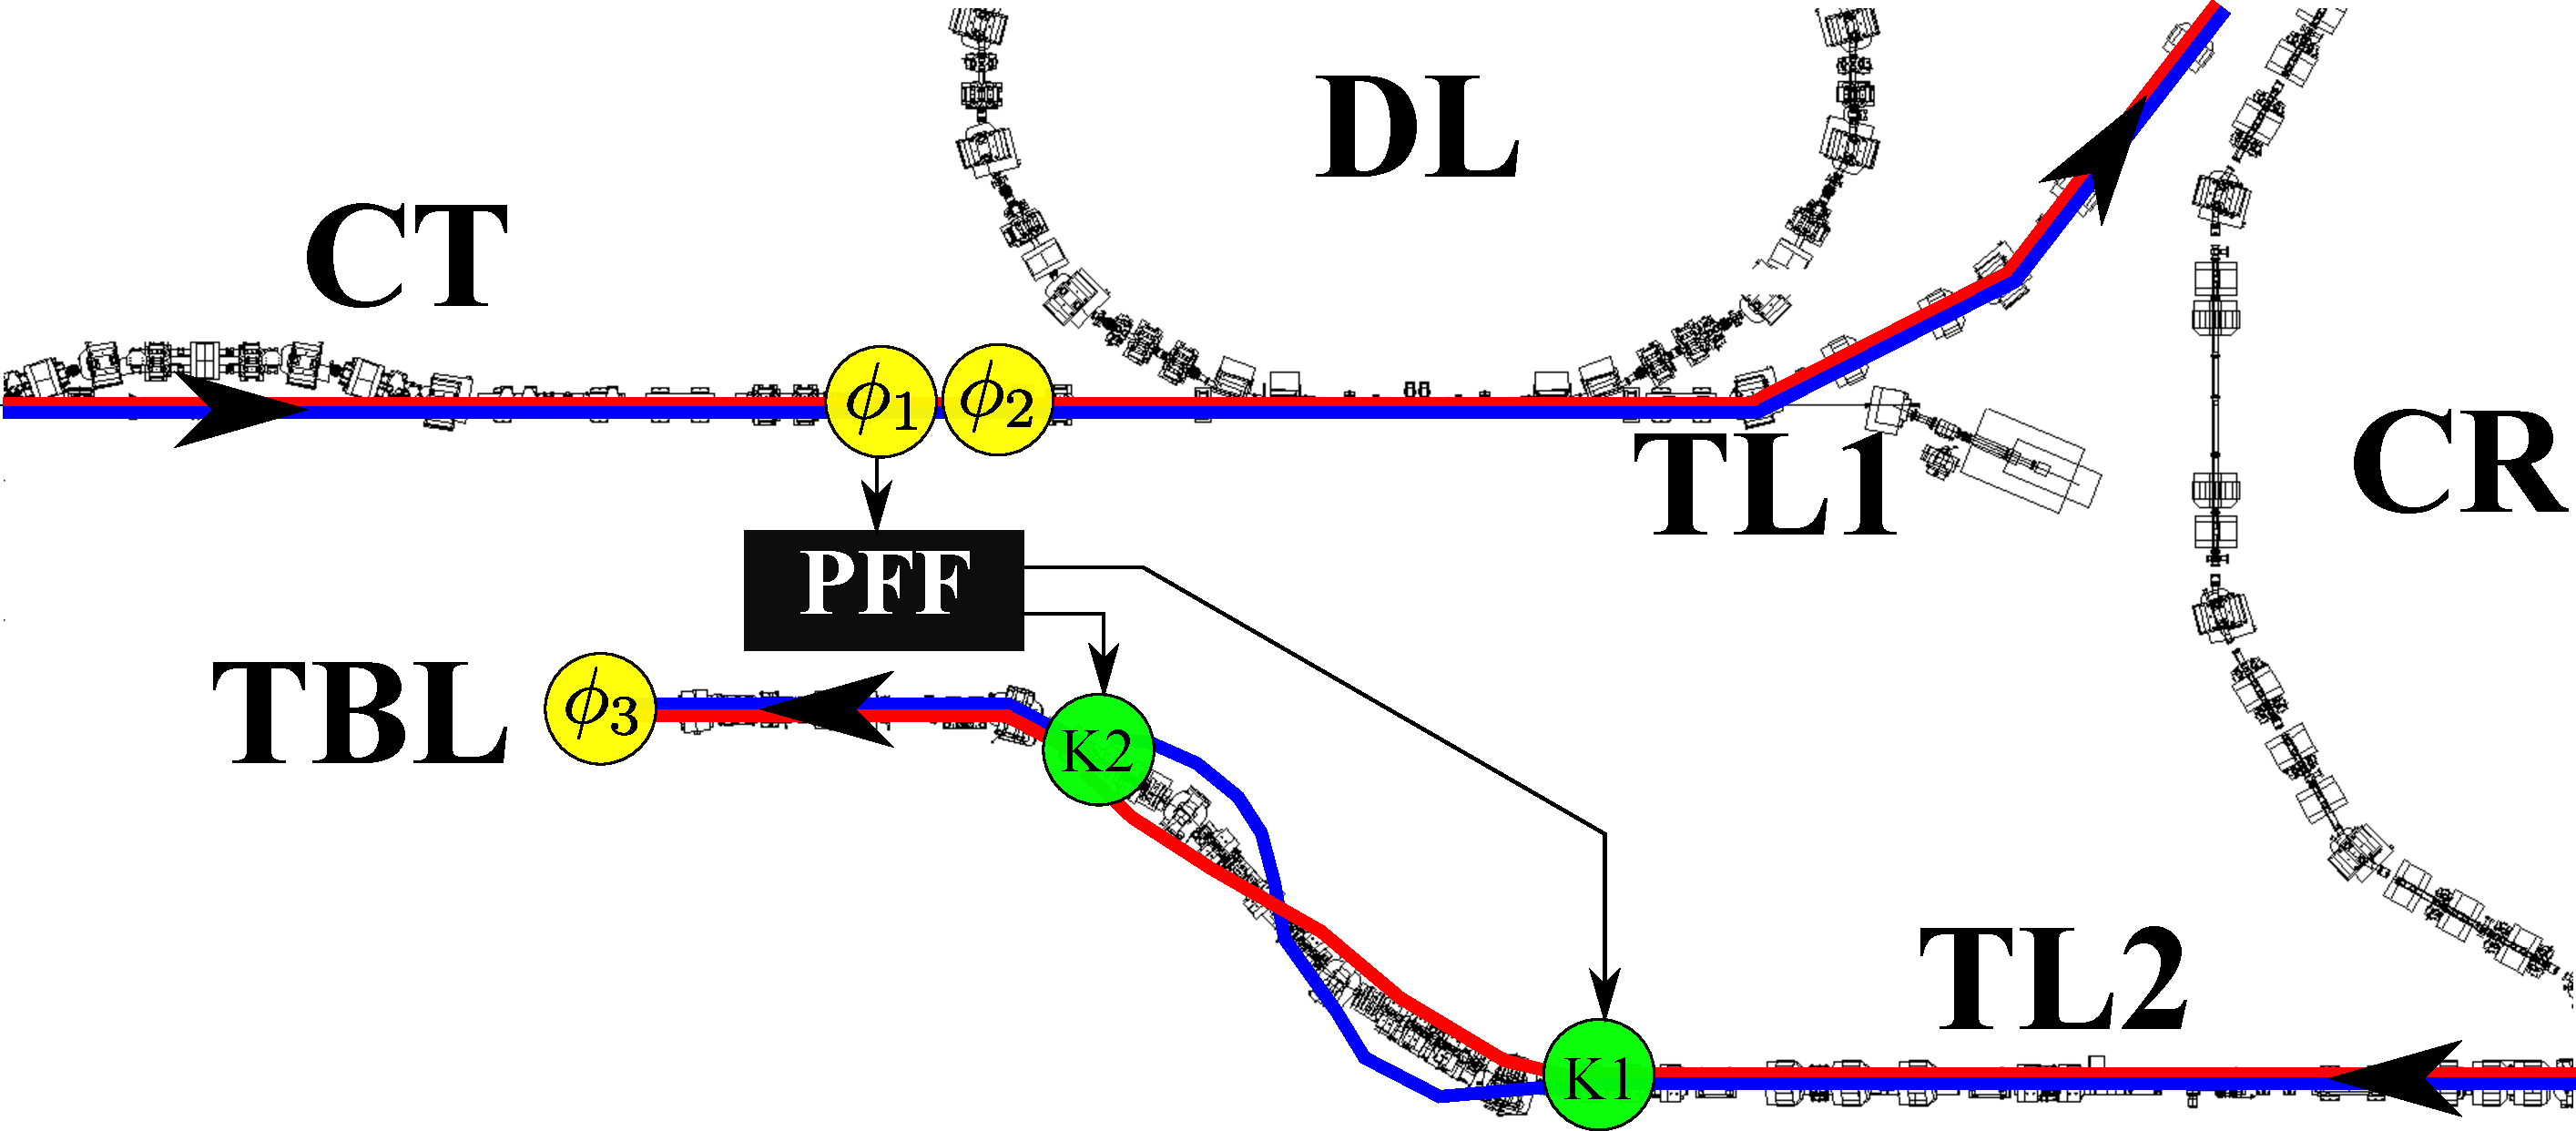
\includegraphics[width=\columnwidth]{figs/ctfpffLayout}% Here is 
	%how to 
	%import EPS art
	\caption{\label{fig:pffLayout}Schematic of the PFF prototype at CTF3, 
	showing the phase monitors (\(\phi_1\) , 
	\(\phi_2\) and \(\phi_3\)) and kickers (K1 and K2). The black box “PFF” 
	represents the calculation and output of the correction, including the 
	phase monitor signal processing electronics, feedforward controller and 
	kicker amplifiers.
	Dashed lines indicate beam lines that are not used during PFF operation. 
		}
\end{figure}

The PFF system presents a significant hardware challenge, in particular in 
terms of the resolution and bandwidth of the phase monitors and of the power, 
latency and bandwidth requirements for the kicker 
amplifiers. A low latency digitiser and feedforward controller is also required.

Table~\ref{tab:pffspecs} compares the requirements of the CLIC system and their 
corresponding values at CTF3. 
The main differences result from the different drive beam energies and scales 
of the two facilities. Higher power amplifiers (500~kW rather than 20~kW) are 
required for CLIC, which may be achieved by combining the output of multiple 
modules similar to those built for CTF3. CLIC also requires the 
synchronisation of multiple PFF systems distributed along the 50~km facility, 
which is not addressed by the CTF3 prototype (see \cite{CLICCDR}).

\begin{table}
	\caption{\label{tab:pffspecs}
	    Requirements for the proposed CLIC PFF system, and how they compare 
	    with the respective CTF3 parameters; performance achieved with the 
	    prototype system is indicated by \textbf{*}.}
\begin{ruledtabular}
	\begin{tabular}{lccc}
		 & CLIC & CTF3 \\
		\hline
		Drive Beam Energy & 2400 & 135 & MeV \\
		No. PFF Systems & 50 & 1 & \\
		Kickers per PFF Chicane & 16 & 2 & \\
		Power of Kicker Amplifiers & 500 & \(\mathbf{20^*}\) & kW \\
		Angular Deflection per Kicker & \(\pm94\) & 
		\(\mathbf{\pm560^*}\) & \(~\mathrm{\mu rad}\) \\
		Correction Range & \(\pm 10\) & \(\mathbf{\pm 6^*}\) & \(^\circ\) \\
		Correction Bandwidth & \(>17.5\) & \(\mathbf{>23^*}\) & MHz \\
		Phase Monitor Resolution & \(< 0.14\) & \(\mathbf{0.12^*}\) &  
		\(^\circ\)   \\
		Initial Phase Jitter & \(2.0\) & \(0.9\) &  \(^\circ\)  \\
		Corrected Phase Jitter & \(0.2\) & \(\mathbf{0.2^*}\) &  \(^\circ\)  \\
	\end{tabular}
\end{ruledtabular}
\end{table}


The phase monitors~\cite{phMonEuCard} are cylindrical cavities with an aperture 
of 23~mm and a length of 19~cm. Small ridges (’notch filters’) in the cavity 
create an effective volume with a resonant frequency of 12~GHz. 
The resonant electromagnetic field induced by the beam traversing the cavity 
contains a beam-position-independent monopole mode and an unwanted 
position-dependent dipole mode. The 
effect of the latter is removed by summing the outputs from an opposing pair 
of feedthroughs, on the top and bottom of the cavity, via an RF ‘hybrid’. 
To extract the beam phase the output from each hybrid 
is mixed with a 12~GHz reference signal derived from a 3~GHz source which is 
time-locked to the CTF3 master oscillator and serves all three phase monitors.
For each phase monitor the beam and reference signals are 
split among an array of eight separate mixers and the outputs are combined to 
give the final phase-dependent signal. A linear response to input beam phase 
was measured over the range \(\pm70^\circ\) \cite{Skowron2013}. By 
comparing the signals from the two adjacent upstream monitors 
(Fig.~\ref{fig:pffLayout}) we have measured~\cite{RobertsThesis} a phase 
resolution of \(0.12^\circ\), i.e. about 30~fs.

The phase signals are digitised  in the feedforward controller (FC) 
board~\cite{RobertsThesis}, which is used to calculate and output the 
appropriate amplifier drive signal. The FC is also used to  control the timing 
of the applied correction. It consists of nine 14-bit analogue to digital 
converters (ADCs) clocked at 357~MHz, a field programmable gate array (FPGA), 
and four digital to analogue converters 
(DACs). 

The kicker amplifiers~\cite{RobertsThesis} have a modular design, 
consisting of a central control module, and two drive and terminator modules 
(one per kicker). The control module distributes power and input signals to the 
drive modules. The 20~kW drive modules consist of low-voltage Si FETs driving 
high-voltage SiC FETs; an input voltage range of \(\pm2\)~V corresponds to an 
output range of \(\pm700\)~V. The response is linear to within 3\% for input 
voltages between \(\pm1.2\)~V, and the output bandwidth is 47~MHz for small 
signal variations of up to 20\% of the maximum. For larger signal variations 
the bandwidth is slew-rate limited.

The two electromagnetic stripline kickers~\cite{kickerIPAC11} are based on the 
DAFNE design \cite{dafnePAC09}. Each kicker is approximately 1~m in length and 
has an internal aperture of 40~mm between the two strips placed along the 
horizontal walls of the device. The kickers are designed to give a fast 
response of a few ns to the input signal. The strips have tapered ends to 
reduce beam coupling impedance. A voltage magnitude of 700~V applied to the 
strips at the downstream end yields a horizontal deflection of 
560~$\mu$rad to the 135~MeV CTF3 beam.

The measured total latency of the phase monitor signal processing, the FC 
calculation, and amplifier response was approximately 100~ns. Therefore the 
output from the FC was delayed by an additional 30~ns to synchronise the 
correction at the kicker with the beam arrival \cite{RobertsThesis}.

\begin{figure}
	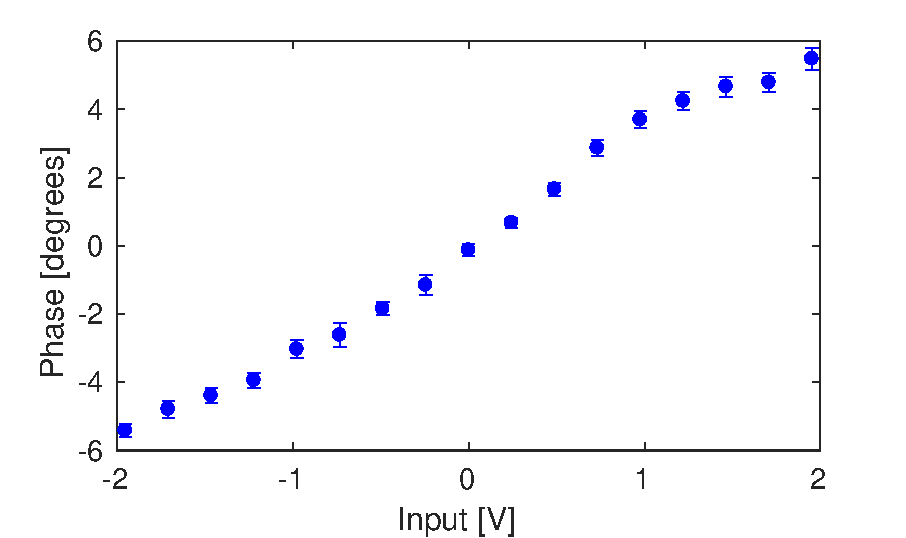
\includegraphics[width=\columnwidth]{figs/corrRange}
	\caption{\label{fig:corrRange}Measured downstream beam phase vs. kicker 
	amplifier input voltage. Standard errors are shown.}
\end{figure}

The operation of the PFF system placed severe constraints on the setting of the 
magnetic lattice in both the beamline between the upstream phase monitors and 
the correction chicane and in  the chicane itself.
The beam transfer matrix coefficient \(R_{52}\) between the two kickers 
characterises the change in path length through the chicane relative to the 
deflection applied at the first kicker. 
With an \(R_{52}\) value of \(0.74\)~m/rad \cite{RobertsThesis} the expected 
maximum path length change for operation of the PFF system, corresponding to 
the maximum deflection of \(\pm560\)~\(\mu\)rad from each kicker, is about 
\(\pm400~\mathrm{\mu m}\), equivalent to \(\pm6^\circ\).
The measured phase shift through the chicane versus the amplifier input voltage 
is shown in Fig.~\ref{fig:corrRange}, and agrees with this expectation. 

In addition, the PFF operation should not change the beam trajectory at 
the exit of the chicane. Therefore the chicane magnet settings were chosen so 
that the second kicker cancels the transverse orbit deviation created by the 
first~\cite{RobertsThesis}.

A further challenge to operation of the PFF was obtaining a high correlation 
between the upstream and uncorrected downstream phases measured at \(\phi_1\) 
and \(\phi_3\) respectively. 
A correlation coefficient of at least 97\% is required to reduce a typical 
incoming phase jitter of \(0.8^\circ\) to the target of \(0.2^\circ\) 
\cite{RobertsThesis}. 
The maximum measurable correlation depends on both the phase monitor resolution 
and any additional phase jitter introduced in the beamlines between \(\phi_1\) 
and \(\phi_3\). The monitor resolution of \(0.12^\circ\) limits the maximum 
upstream-downstream phase correlation to \(98\%\) in typical conditions, and 
places a theoretical limit of \(0.17^\circ\) on the measurable corrected 
downstream phase jitter. 
The dominant source of uncorrelated downstream phase jitter arises from  
beam energy jitter that is transformed into phase jitter. 

\begin{figure}
	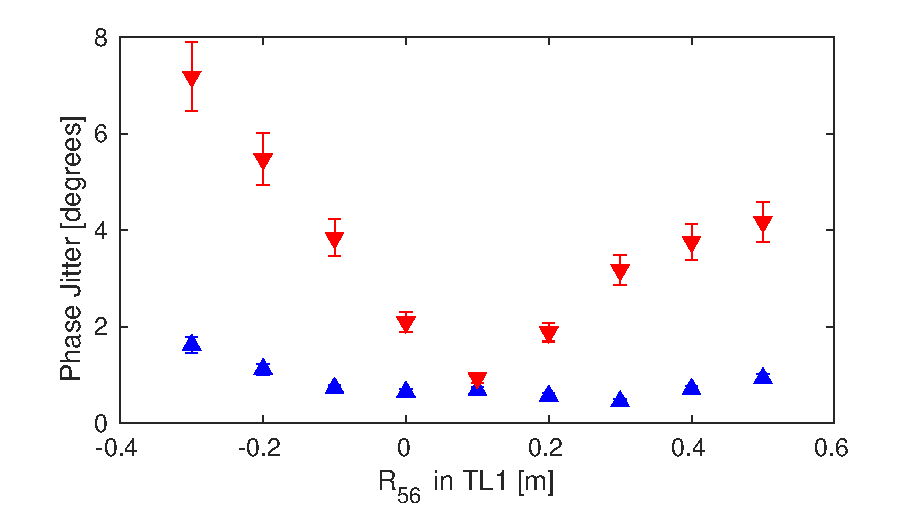
\includegraphics[width=\columnwidth]{figs/r56Scan}
	\caption{\label{fig:r56Scan}Measured downstream (red) and upstream (blue) 
	phase jitter vs. TL1\(R_{56}\) value. Standard errors are shown.
		}
\end{figure}

To first order the phase-energy dependence can be described via the beam 
transfer matrix coefficient 
\(R_{56}\):
\(\phi_3 = \phi_1 + R_{56}(\Delta p / p)\)
, where \(\Delta p / p\) is the relative beam energy offset.
The optimal condition is \(R_{56}\) = 0.
This was achieved by tuning the \(R_{56}\) value in the `TL1' transfer line 
so as to compensate for non-zero \(R_{56}\) in the other beamline sections
(Fig.~\ref{fig:r56Scan}). With \(R_{56}\) = 10~cm in TL1 the 
downstream phase jitter is reduced to the same level as the upstream jitter. 
However, a large second-order phase-energy dependence remained uncorrected, 
resulting in a degradation in upstream-downstream phase correlation if there 
are drifts in beam energy.

The performance of the PFF correction is controlled by a ‘gain’ parameter. 
%\begin{equation*}
%\sigma_{\mathrm{PFF}}^2 = \sigma_d^2 + g^2\sigma_u^2 - 
%2g\rho_{ud}\sigma_u\sigma_d
%\end{equation*}
Theoretically the best gain, in appropriate units, should 
be roughly unity, but in practice the gain can be chosen to achieve optimal 
performance for real beam conditions. A representative gain scan is shown 
in~Fig.~\ref{fig:gScan}; the optimal gain was typically found to be near 
unity. For beam conditions in which there is a small amplification in the 
downstream phase jitter with respect to the upstream phase jitter a gain 
slightly above unity provides the best achievable phase-jitter reduction
\cite{RobertsThesis}. At CTF3 the optimal system gain is typically in the range 
1.0--1.2.
Also shown in Fig.~\ref{fig:gScan} is a theoretical prediction of the corrected 
phase jitter considering the initial beam conditions; the phase jitter at 
\(\phi_1\) and \(\phi_3\) and the upstream-downstream phase correlation. The 
simulation reproduces the data.

\begin{figure}
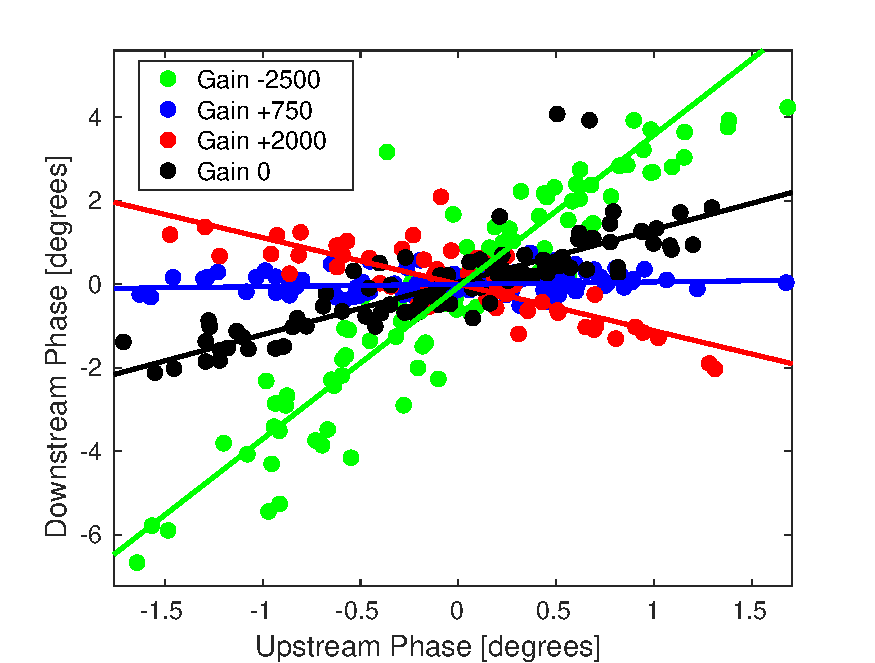
\includegraphics[width=\columnwidth]{figs/gScan}
\caption{\label{fig:gScan}Measured corrected beam  phase jitter at $\phi_3$ vs. 
PFF gain; standard error are shown (points). The theoretically-achieveable 
performance is shown by the red shaded region (see text).}
\end{figure}

In order to meet CLIC requirements (Table~\ref{tab:pffspecs}) the PFF 
correction bandwidth should be at least 17.5 MHz so as to allow correction 
within the 240ns-long drive-beam pulse. This function was tested with the CTF3 
prototype, which was used to remove phase variations within a portion of the 
1.2~\(\mathrm{\mu s}\) CTF3 beam pulse (Fig.~\ref{fig:shape}).  It is an 
operational feature at CTF3 that there is a roughly parabolic phase sag of 
\(40^\circ\) peak-to-peak, 
resulting from the upstream RF pulse compression scheme~\cite{CLICCDR}. Hence 
approximately a 440~ns portion of the pulse is within the \(\pm 6^\circ\) 
dynamic range of the PFF system for the duration of a 30~minute dataset, and 
can be corrected to zero nominal phase. 
This time duration for the full correction exceeds the CLIC drive-beam pulse 
length of 240ns and in any case the CLIC design avoids such 
a large phase sag~\cite{CLICCDR} 

\begin{figure}
	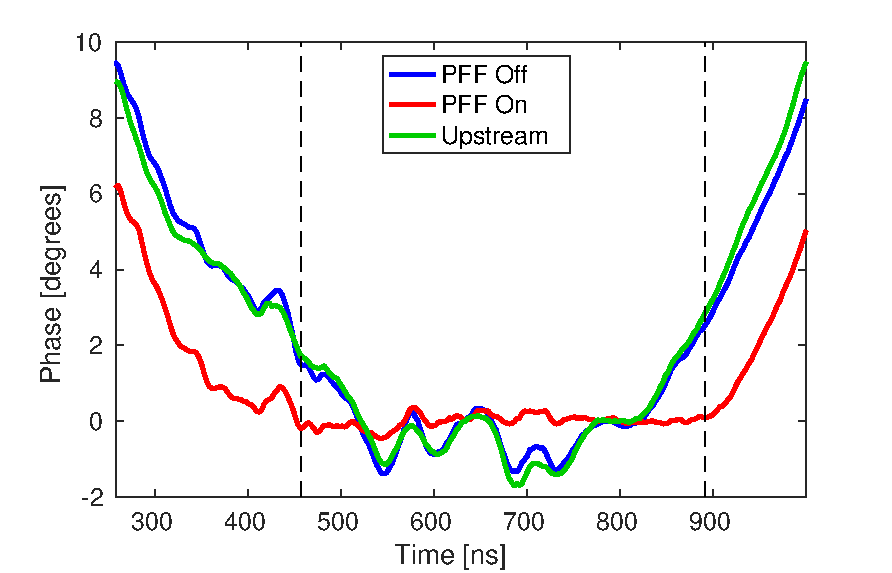
\includegraphics[width=\columnwidth]{figs/shape}
	\caption{\label{fig:shape}Phase vs. time within the central portion of the 
	CTF3 beam pulse. The traces show the incoming phase measured in \(\phi_1\) 
	(green) and the downstream phase measured in \(\phi_3\) with PFF off (blue) 
	and PFF on (red). Each trace is the average across the 30 minute dataset.
	The vertical dashed lines mark the time interval corresponding to the PFF 
	dynamic range. }
\end{figure}

Fig.~\ref{fig:shape} shows the effect of the PFF system on the intra-pulse 
phase variations. The convention at CTF3 is to 
operate the PFF system in interleaved mode, with 
the correction applied to alternating pulses only. This allows a measurement of 
the initial (`PFF Off') and corrected (`PFF On') downstream phase to be 
performed concurrently. The upstream (PFF input) phase is also shown for 
comparison. Vertical dashed lines mark the 440~ns portion of the pulse where 
the 
correction is optimal, and this range is used in all analyses of the 
effect of the system. 

Within this range the PFF system flattens the phase, 
and almost all variations are removed. Residual offsets in the phase are still 
present where there are small uncorrelated differences between the shapes of 
the incoming upstream and downstream phases. 
The average rms phase variation within the 440~ns window is reduced from 
\(0.960\pm0.003^\circ\) with the PFF system off, to \(0.285\pm0.004^\circ\) 
with the system on.

\begin{figure}
	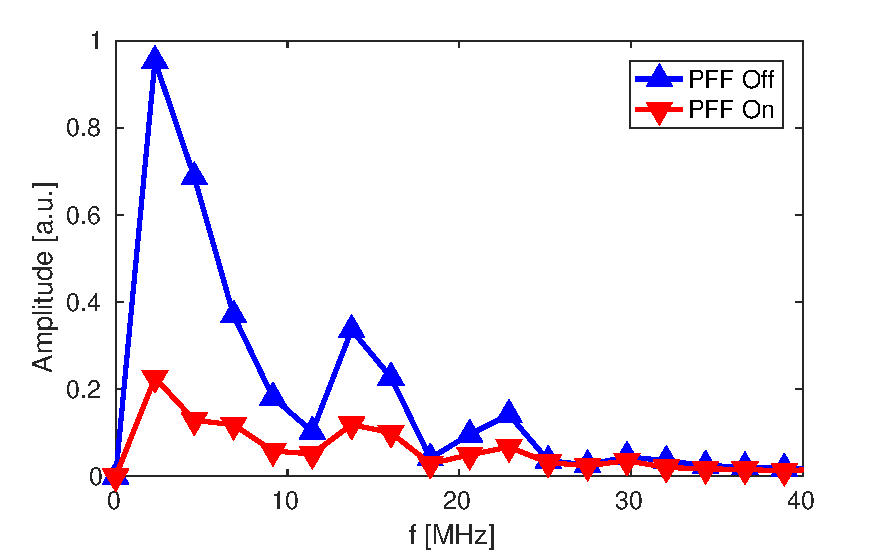
\includegraphics[width=\columnwidth]{figs/fft}
	\caption{\label{fig:fft}Amplitude of phase errors at different frequencies 
		(\(f\)) with the PFF system off (blue) and on (red).}
\end{figure}

A Fourier-Transform (FFT) method was used to characterise the PFF on/off 
datasets. The FFT amplitude is shown vs. frequency in 
Fig.~\ref{fig:fft}. It can be seen that phase errors are corrected by up to a 
factor of 5 for frequencies up to 23~MHz, above which 
phase errors are smaller than the monitor resolution and not measurable. This 
is consistent with an expected system bandwidth of around 30~MHz.

As well as removing intra-pulse phase variations the PFF system simultaneously 
corrects any pulse-to-pulse jitter. For each beam pulse the mean phase is 
calculated as the average across the 440~ns window in Fig.~\ref{fig:shape}.

Fig~\ref{fig:meanJit} shows the effect of the PFF system on the mean 
phase stability for a dataset of around ten minutes duration.
The pulse-to-pulse phase jitter is reduced from  \(0.92\pm0.04^\circ\) to 
\(0.20\pm0.01^\circ\) by the PFF correction, demonstrating CLIC-level phase 
stability. 
The PFF system acts to remove all correlation between the upstream and 
downstream phase, reducing an initial correlation of \(96\pm2\%\) to 
\(0\pm7\%\) for this dataset.
Given the incoming upstream phase jitter and 
measured upstream-downstream correlation, the performance is consistent with 
the theoretically predicted correction of \(0.26\pm0.06^\circ\).

\begin{figure}
	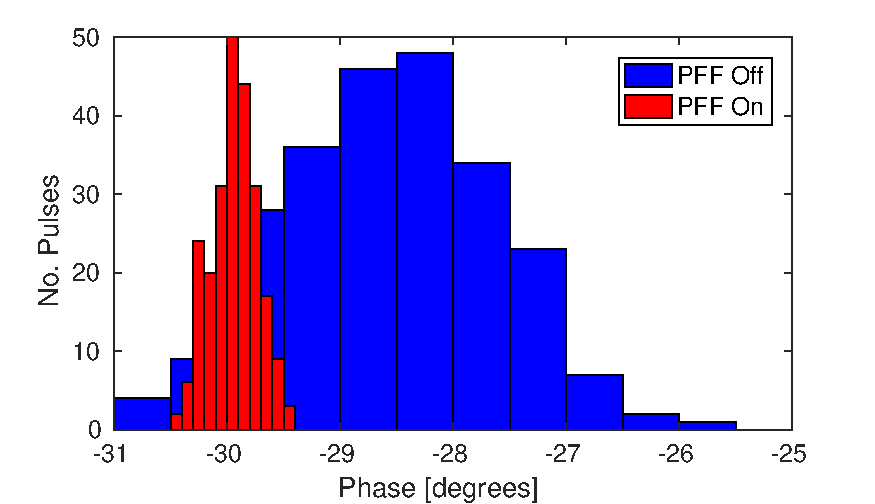
\includegraphics[width=\columnwidth]{figs/meanJit}
	\caption{\label{fig:meanJit}Distribution of the mean downstream phase with 
		the 
		PFF system off (blue) and on (red).}
\end{figure}

Typically this level of corrected phase stability could not be maintained for 
longer time periods due to drifts in the operation of the CTF3 RF system, which 
led to  a degradation in the upstream-downstream phase correlation as well as 
mean phase drifts beyond the PFF correction range. Nevertheless a mean phase 
stability of \(0.30^\circ\) was achieved in datasets taken over periods as long 
as 20~minutes. With suitable upstream RF feedbacks to keep the beam phase 
within the correction range, and a reduction of the higher order phase-energy 
dependence in the magnetic lattice, the PFF system is capable of achieving 
CLIC-level phase stability continuously.

The PFF system was further tested by intentionally varying the incoming mean 
beam phase systematically by up to \(3^\circ\); such a variation is comparable 
to the expected conditions in the CLIC design (Table~\ref{tab:pffspecs}). 
This is illustrated in (Fig.~\ref{fig:wiggle}). The system removed the induced 
phase variations and achieved more than a factor-5 reduction in the downstream 
phase jitter, correcting from \(1.71\pm0.07^\circ\) to \(0.32\pm0.01^\circ\). 

\begin{figure}
	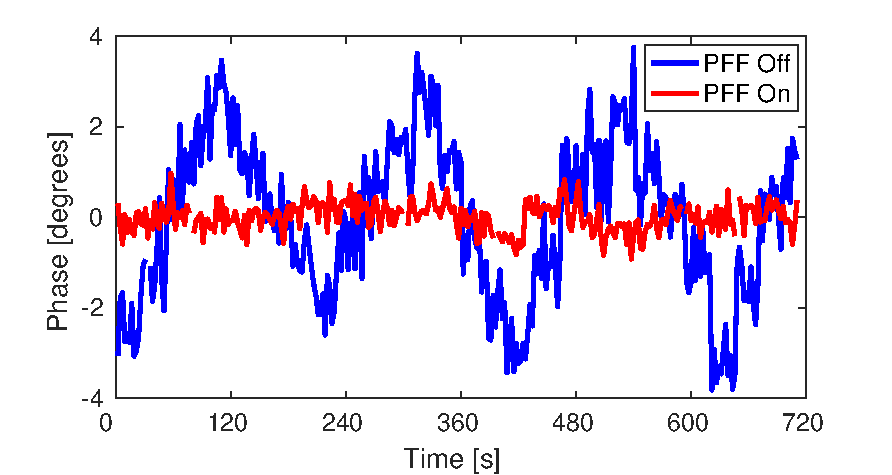
\includegraphics[width=\columnwidth]{figs/wiggle}
	\caption{\label{fig:wiggle}Mean downstream phase vs. time with the PFF 
	system off (blue) and on (red) subject to large additional phase variations 
	added to the incoming phase (see text).}
\end{figure}

%%%%%%%%%%%%

In conclusion, we have built, deployed and tested a prototype drive-beam phase 
feedforward system for CLIC.   The system incorporates high-resolution phase 
monitors, an advanced signal-processor and feedforward controller, low-latency, 
high-power, high-bandwidth amplifiers, and state-of-the-art electromagnetic 
kickers. The phase-monitor resolution was measured to be 
\(0.12^\circ\simeq\)~30~fs.  The overall system latency, including the hardware 
and 
signal transit times, was measured to be approx. 350~ns, which is less than 
beam time of flight between the input phase monitor and the correction 
chicane.  Therefore, the feedforward phase correction was applied downstream to 
the same beam bunches initially measured upstream.

The prototype system was used to stabilise the pulse-to-pulse  
phase jitter to \(0.20\pm0.01^\circ\simeq\)~50 fs. It also simultaneously 
corrected intra-pulse phase variations up to a frequency of 23~MHz. 

%\begin{acknowledgments}
%	We thank Alessandro Zolla and Giancarlo Sensolini (INFN 
%	Frascati) for their work on the mechanical design of the phase monitors and 
%	kickers, 
%	Alexandra Andersson, Luca Timeo and Stephane Rey (CERN) for their work on 
%	the phase monitor electronics. We thank the operations team of 
%	CTF3 for their outstanding support. We acknowledge the UK Science and 
%	Technology Facilities Council for their financial 
%	support for this work. \end{acknowledgments}

\bibliography{pff_short}

\end{document}
